\documentclass[12pt]{article}
\title{Discouragement Attacks}
\author{
        Vitalik Buterin \\
        Ethereum Foundation
}
\date{\today}
\usepackage{graphicx}


\begin{document}
\maketitle
\begin{abstract}
We explore ``discouragement attacks" on economic consensus mechanisms. A discouragement attack consists of an attacker acting maliciously inside a consensus mechanism in order to reduce other participants' revenue, even at some cost to themselves, in order to encourage the victims to drop out of the mechanism. The motivations to conduct discouragement attacks are twofold. First, the attacks can increase the attacker's profit, as the mechanism may contain long-run ``competitive" mechanics where some participants dropping out increases revenue to the remaining ones. Second, the attacks can be part of a two-step strategy where the second step is to carry out a traditional $51\%$ attack on the consensus algorithm against a now much smaller set of ``honest" participants warding off the attacker, and hence pay a much lower cost for the attack.
\end{abstract}

\section{Introduction}
We model an economic consensus mechanism as being a game where there is an infinite set of participants each with an infinitesimally small deposit (we'll call the ``size" of the set the total sum of deposits), of which some portion is controlled by the attacker. The payout function takes as input $x$, the total size of the participant set, and $h$, the extent to which the attacker deviates from an ``honest" strategy. The payout to each honest participant is $\frac{1-h}{x^p}$, where $p$ is a protocol parameter that determines how the protocol reward changes with the number of participants. For example:

\begin{itemize}
\item $p=0$: constant ``interest rate", eg. under optimal conditions each participant earns a return of $8\%$ per year.
\item $p=\frac{1}{2}$: the rewards (and penalties) to participants scale with the inverse square root of the size of the participant set, so \textit{total} rewards scale with the square root of the size of the participant set. This is a compromise between $p=0$ and $p=1$. 
\item $p=1$: constant total reward, ie. the total payout of the protocol is dependent only on what percentage of participants take what actions, not on the size of the participant set. 
\item $p=\infty$: the protocol is dead-set on ensuring that the total size of the participant set is some specific constant $k$ no matter what. If the size exceeds $k$, the protocol keeps decreasing rewards until the size drops to $k$, and if the size is below $k$, the protocol keeps increasing rewards until the size rises to $k$.
\end{itemize}

Note that if revenues to participants are dominated by transaction fees, then $p=1$ will hold.

Each participant controlled by the attacker pays $\frac{1-\frac{h}{r}}{x^p}$ where $r$ is the \textit{proportional loss ratio}. The proportional loss ratio is the ratio between the loss the victims suffer and the loss the attacker suffers, where both losses are expressed in percentage terms. For example, if an attack that causes the attacker to lose $1\%$ of deposits of all participants that they control causes everyone else to lose $2\%$, then the proportional loss ratio is 2.

The reason behing the above formulas is as follows. We assume that there is some ``base interest rate'' paid to all participants, which is proportional to some inverse power of the total size of the participant set. There is not necessary a principled in-protocol notion of the ``extent'' to which an attacker is attacking, so we define our own: the extent of an attack is $h$ if the victims' return decreases to $\frac{1-h}{x^p}$. We assume the proportional loss ratio $r$ is fixed, hence the attacking participants' return must be $\frac{1-\frac{h}{r}}{x^p}$.

In contracts the \textit{griefing factor}, another way of comparing attacker and victim losses, is defined in absolute terms: for example, if in such a scenario the attacker controls $\frac{1}{3}$ of the total participant set, then the set of victims is twice as large as the attacker, and so altogether the victims lose four times more than the attacker, and so the griefing factor would be 4. The relationship between the proportional loss ratio $r$ and griefing factor is simple: $$g = r * \frac{1-\alpha}{\alpha},$$ where $\alpha$ is the portion of participants controlled by the attacker. In our above example, $\alpha = \frac{1}{3}$, so $g = 2 * \frac{\frac{2}{3}}{\frac{1}{3}} = 4$.

We now rephrase the problem into the language of supply and demand: there exist a set of players, each of which has some \textit{reserve interest rate} at which they are willing to become participants in the consensus mechanism. This is the demand curve, where the interest rate is the price. The protocol, which offers interest rates for participation in the consensus mechanism, sets the supply curve. If $p=0$, the supply curve is horizontal - the protocol offers that interest rate to an unlimited number of participants. If $p=\infty$, the supply curve is vertical. For any other $p$, the supply curve is declining with a constant elasticity of $\frac{1}{p}$. We model the attacker as having unilateral power to set $h$ (by attacking), and this pushes down the supply curve.

We model the demand curve as also being a simple exponential function, $x^d$. In general, we expect there to be wide disparities between the reserve interest rates of different players, as they have different levels of wealth, technical capability to operate a node in the consensus mechanism, and willingness to lock up their capital; additionally, we expect many players will be readily willing to lock up $50\%$ of their capital, somewhat willing to lock up $80\%$, hard pressed to lock up $95\%$, and not willing at all to lock up $100\%$. Hence, $d > 1$ seems likely, though we will consider the problem abstractly and give results for various values of $d$.

\section{Analysis}

We want to learn two things. First, are there opportunities to perform a discouragement attack for profit? Second, what is the difficulty of performing a discouragement attack in order to set up a cheaper later attack on consensus? To examine the second case, we can compare the pre-discouragement and post-discouragement intersections of the supply and demand curves.

Pre-discouragement, the intersection is between $y = \frac{1}{x^p}$ and $y = x^d$. The unique solution is clearly $x=1$ and $y=1$. Note that we can adjust the currency unit and the time unit so that the default equilibrium of 1 unit and an interest rate of $100\%$ per period holds; hence, the omission of adjustable constants in the supply and demand curve formulas does not sacrifice generality.

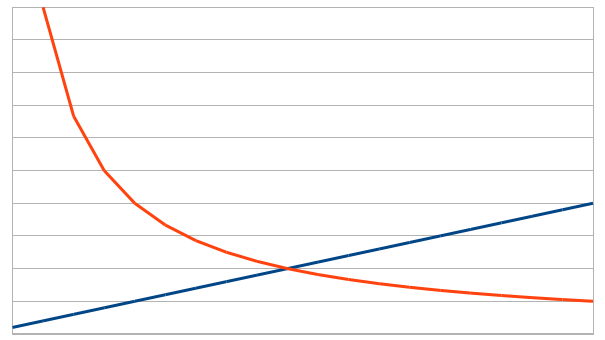
\includegraphics[width=300px]{disc_chart1.png}

Post-discouragement, it becomes:

$\frac{1-h}{x^p} = x^d$

$x=(1-h)^{\frac{1}{d+p}}$

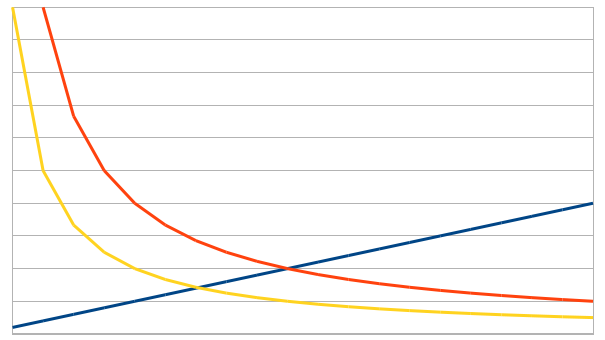
\includegraphics[width=300px]{disc_chart2.png}

Let us now look at the attacker's interest rate, $\frac{1-\frac{h}{r}}{x^p}$. First, let us take the easy case: $r \le 1$. In this case, $\frac{1-\frac{h}{r}}{x^p} \le \frac{1-h}{(1-h)^{\frac{p}{d+p}}} = (1-h)^{\frac{d}{d+p}} < 1$. Hence, if $r \le 1$, the attacker will always lose money. This may seem counterintuitive; one might ask, what if the discouragement attack pushes out so many other participants that the new equilibrium is on the very high part of the the supply curve close to zero? The important thing to keep in mind, however, is that if $r = 1$ (i.e. the attacker gets the same interest rate as the victims), then the attacker's revenue will necessarily be at some point along \textit{the original, unchanged, upward sloping demand curve}. Because the demand curve is upward sloping, and the number of participants decreased, the interest rate paid to the attacker must have also decreased. If $r < 1$, then the attacker loses \textit{even more} than the victims, at least if expressed as an interest rate, and so the attacker's interest rate will end up \textit{below} the lower point along the demand curve experienced by victims. Hence, if $r \le 1$, discouragement attacks are necessarily costly.

In general, it is certainly feasible to design a consensus mechanism where we can ensure $r \le 1$ as long as the attacker controls less than $50\%$ of participants, so this is already a very useful result. Now, let us examine the case where $r > 1$. For very high values of $r$, it is easy to see how the attacker can theoretically make a net gain from a discouragement attack:

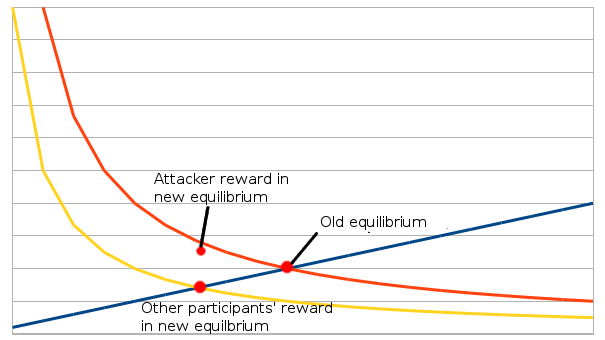
\includegraphics[width=300px]{disc_chart3.png}



However, with the right bounds we can still prevent such an attack from being profitable. Consider the case where $p=1$, and where the attacker must maintain a $50\%$ share of active participants to exert $r > 1$ griefing (note that at the $50\%$ boundary, the \textit{proportional loss ratio} $r$ and the \textit{griefing factor} are the same value). The next question is, does the attacker remove some of their own participants to keep their share at $50\%$, or do all of the participants controlled by the attacker stay?

In the first case, as long as $r \le 1$, no matter how high $r$ is, the attacker's revenue must still decrease, or in the worst case where $r = \infty$, the attacker's revenue will be unchanged. In the second case, we note that the size of the participant set will decline more slowly - specifically, $x = \frac{1}{2} + \frac{1}{2} * (1-h)^{\frac{1}{d+p}}$. Suppose $r \le 2$, and $p \le 1$. Then:

$\frac{1-\frac{h}{r}}{x^p}$


$ \le \frac{1-\frac{h}{2}}{(\frac{1}{2} + \frac{1}{2} * (1-h)^{\frac{1}{d+p}})^p}$
$ \le \frac{1-\frac{h}{2}}{\frac{1}{2} + \frac{1}{2} * (1-h)^{\frac{p}{d+p}}}$
$ = \frac{\frac{1}{2} + \frac{1}{2} * (1-h)}{\frac{1}{2} + \frac{1}{2} * (1-h)^{\frac{p}{d+p}}}$
$ \le \frac{\frac{1}{2} + \frac{1}{2} * (1-h)}{\frac{1}{2} + \frac{1}{2} * (1-h)}$
$ = 1$
Hence both strategies are unprofitable. For values $r > 2$, the proof would need to be more conditional on specific values of $p$. We can make the claim that, if the griefing factor is bounded by $GF$, i.e. $r \le GF * \frac{\alpha}{1-\alpha}$, then a discouragement attack cannot be profitable if and only if $p \le \frac{1}{GF}$.

We can check this at the boundary $h = 1$ as follows. We want to show that $\frac{1 - hp * \frac{1-\alpha}{\alpha}}{(\alpha + (1-\alpha)(1-h)^{\frac{d}{d+p}})^p} \le 1$, so we show that the numerator is less than or equal to the denominator. At $h = 1$, the numerator simplifies to $1 - \frac{p}{\alpha} + p$ and the denominator to $\alpha^p$. At $\alpha=1$, the two are equal. To show that the numerator is strictly less for $\alpha<1$, we can take the derivative of both with respect to $\alpha$; the numerator becomes $\frac{p}{\alpha^2}$ and the denominator becomes $p * \alpha^{p-1}$, and since $\alpha < 1$ the derivative of the numerator is clearly greater, so for $\alpha < 1$ the original fraction will be less than one. Checking for $0 < h < 1$ is much harder, but analytically it can be verified that it holds.

Hence, if the griefing factor is bounded by 2, we want $p \le \frac{1}{2}$, and similarly for other griefing factors.


\section{Discouragement Attacks for Breaking Consensus}

Here we evaluate the feasibility of attackers with a two-step plan. First, run a discouragement attack to push other participants out. Second, attack the network against a now much smaller participant set. The second attack could either be a finality reversion attack, or it could be censorship. In the given model, this is clearly doable: an attacker can grief with $h > 1$ to push all other participants out, then remove most of their own participants, then use the remainder to perform the attack. This can be overcome with an honest minority assumption, where some participants are willing to stay despite the lack of economic incentive, and it can also be overcome with outside donations to ``honest" participants. A third way that it can be overcome is if, when such an attack starts taking place, a large number of outside players temporarily join the participant set, diluting the attacker to below $50\%$ and thereby making their attack ineffective.

This kind of attack is difficult to economically model because under certain assumptions the cost is zero: if an attacker can credibly announce that they will grief with $h > 1$, then all other participants will leave, and the attacker will then be free to join with one single participant and perform a censorship attack at infinitesimal cost. This result is true in \textit{any} game where the net profit of a participant can be made to drop below zero through no fault of their own, which is itself true of any consensus algorithm where a censorship attack has nonzero cost, because of the fundamental fault inattributability of censorship versus a minority going offline.

What we \textit{can} do is model the game in various ways that add realistic ``friction" to non-attacking participants' economic reasoning, and see how the parameters of the game can be optimized so as to maximize the cost of attack given these frictions. One possibility is to model it as a three-phase game, where in phase 1 the attacker griefs with some $h$, all participants get their due rewards and penalties ($y_0 * (1 - h)$ for the attacker, $y_0 * (1- r * h)$ for everyone else, where $y_0 = \frac{1}{x_0^p}$ is the default``peacetime" interest rate), then in phase 2 both the attacker and other participants make choices about how to allocate their resources and finally in phase 3 the attacker decides whether or not to attack. The attacker is modeled as having a \textit{budget} $b$; the attacker is only willing to lose $b$ in order to carry out the attack.

Let us first consider finality reversion attacks. In a finality reversion attack, if the total validator set has size $x$, the cost of an attack is $\frac{x}{3}$. An attacker's strategy is easy: grief with $h = \frac{1}{r}$ in phase 1, drive all other participants away as their revenue drops to zero, and then attack in phase 2. The attacker's cost here, assuming the attacker had $50\%$ of the validator set in phase 1, is $x_0 * \frac{1}{2} * (1 - \frac{1}{r})$.

Now, let us modify the game slightly: suppose that of the $\frac{x}{3}$ penalized, half goes to all other participants. Suppose the total validator set has size $x_1$ in phase 1, with base interest rate $y_1 = \frac{1}{x_1^p}$. The attacker griefs with some $h$ in phase 1, and as a result in phase 2 the validator set drops in size to $x_2$, with base interest rate $y_2 = \frac{2}{x_2^p}$. The attacker then attacks with probability $P_{attack}$.

The attacker's cost is:

$\frac{1}{2} * x_1 * y_1 * h + P_{attack} * \frac{1}{3} * x_2$

The first term in the sum is the cost in phase 1, and the second term is the expected cost in phase 2.

Supply-demand equilibrium tells us that in phase 2 we have:

$y_2 * (1-h) + \frac{1}{4} * P_{attack} = x_2^d$

The $\frac{1}{4}$ fraction comes from the fact that during an attack, non-attacker's deposits would increase by 25\%. Let us assume $d = p = 1$. We can simplify:

$\frac{1}{x_2} * (1-h) + \frac{1}{4} * P_{attack} = x_2$

This gives us $x_2$ out of $P_{attack}$ and $h$ through a quadratic equation, which we can then plug into the attacker's cost. If we normalize $x_1 = y_1 = 1$, then this gives the cost as a function of $h$ and $P_{attack}$. The quadratic equation is:

$x_2 = \frac{\frac{P_{attack}}{4} + (\frac{P_{attack}^2}{16} - 4 * (h-1))^{\frac{1}{2}}}{2}$

Let's look at the case $P_{attack} = 1$. Then, $x_2 = \frac{\frac{1}{4} + (\frac{1}{16} - 4 * (h-1))^{\frac{1}{2}}}{2}$. The discriminant equals zero when $h = \frac{65}{64}$, and for higher values of $h$ the discriminant goes negative. Hence, for any value of $h$ substantially above 1, there is no solution, suggesting that there is no $x_2$ at which participants would find it profitable to stay. This can be seen as a negative feedback loop: the lower $x_1$ goes, the more highly negative the interest rate can go, and so $x_1$ goes further down. This suggests a rationale for designing the mechanism so that the maximum possible $h$ is lower the lower the size of the participant set, until below some critical size it is not much lower than 1. Additionally, it is also an argument for selecting lower values of $p$, though the benefit is fairly marginal.

In general, what this analysis suggests is that (i) discouragement attacks for consensus breaking are difficult to fully defeat, (ii) setting lower values of $p$ is a good idea, and (iii) perhaps the best way to is to increase friction for participants in the consensus game looking to drop out.

\section{Bribing to counter-grief}

Suppose that victims ($\le 50\%$ of the participant pool) are concerned that their revenue will decrease from $y_0$ to 0 as part of a discouragement attack. They can choose to bribe outsiders to enlist in order to prevent this from happening. Bribing outsiders individually is expensive, because the bribe must overcome the outsider's concern that they themselves will suffer from the attack. However, with an assurance contract we can create a bribe that only works if enough outsiders show up. A bribe to increase the participant set by a factor of $n$ would cost $(n - 1) * (n^d - \frac{1}{n^p})$. If $p = d = 1$, this equals $n * (n - \frac{1}{n}) = n^2 - 1$. Hence, such a bribe would be rational to organize if $n \le \sqrt{2}$.

However, suppose that participants fear not just loss of profits, also heavy losses, because they believe that an attacker will launch an attack and destroy a large portion of their deposits. Then, $n$ can be increased further, especially if the choice is between a small change between already relatively low interest rates and a large short-term harm of losing a large portion of one's deposit. To assist this mechanism, it is worth considering paying a small interest rate to those who are not participating in the consensus game, but are willing to make their deposits ``conscriptable", in the sense that they automatically join the consensus game as soon as some condition is triggered (for example, net interest rates including penalties dropping below zero).


\section{Conclusion}

Discouragement attacks as a cheaper way of attacking a consensus algorithm are one of the hardest classes of attacks to come up with defenses against. This is true in proof of work as well: if a 51\% attack succeeds, then there is a coordination problem opposing ``honest" miners trying to recover the original fork, as none have the private incentive to participate in a fork unless everyone else does. Hence, our recommendations at this point can consist only of two parts. First, there exist marginal tweaks that can be made to mechanisms to reduce the effectiveness of discouragement, increasing difficulty of leaving the validator pool and keeping $p$ values low (particularly by not relying solely on transaction fees) being chief among them. Second, if a discouragement attack does start happening, expect an assurance contract bringing in more participants to be an important building block in the solution.

In general, this is still an active area of research, and more research in counter-strategies is desired.

\bibliographystyle{abbrv}
\bibliography{main}

\end{document}
